\documentclass{article}
\usepackage{graphicx}
\usepackage{float}
\begin{document}
\title{Malwares for Use cases for EMI measurements}
\author{Abhinav Narain}
\maketitle

\section{Purpose}
The purpose of the document discusses Alexa and Nest camera EMI to
for representing device activity/state. It does not have Google Home
results as no purchases were made after multiple requests in past weeks.

It further discusses some real-world workload, crypto-currency miners
on IoT and related experiments. Follow up on reaching out few
hackers/reversers to seek malware codebase.

\textit{Note}: Time is measured in seconds in all the spectrograms.
\section{Nest Camera}
The following observations on the spectrograms are worth noting:
\begin{enumerate}
\item There is a difference in a faint band present at 100 KHz
  frequency when the camera is turned On (from
  mobile app in Figure~\ref{fig:nest_stream}) vs when it is in standby mode (streaming video turned
  off).
\item The band is more prominent when a higher resolution video is
  chosen in Figure~\ref{fig:nest_standby}
  \item EMI intensity increases for higher resolution
    camera (in Figure~\ref{fig:nest_stream1080} of 1080) vs default
    resolution (in Figure~\ref{fig:nest_stream})
\item I am not sure about a perceivable change when the
  audio (in Figure~\ref{fig:nest_stream_audio}) with camera is On vs silent
  default streaming (in Figure~\ref{fig:nest_stream})
\end{enumerate}

\begin{figure}[H]
\centering
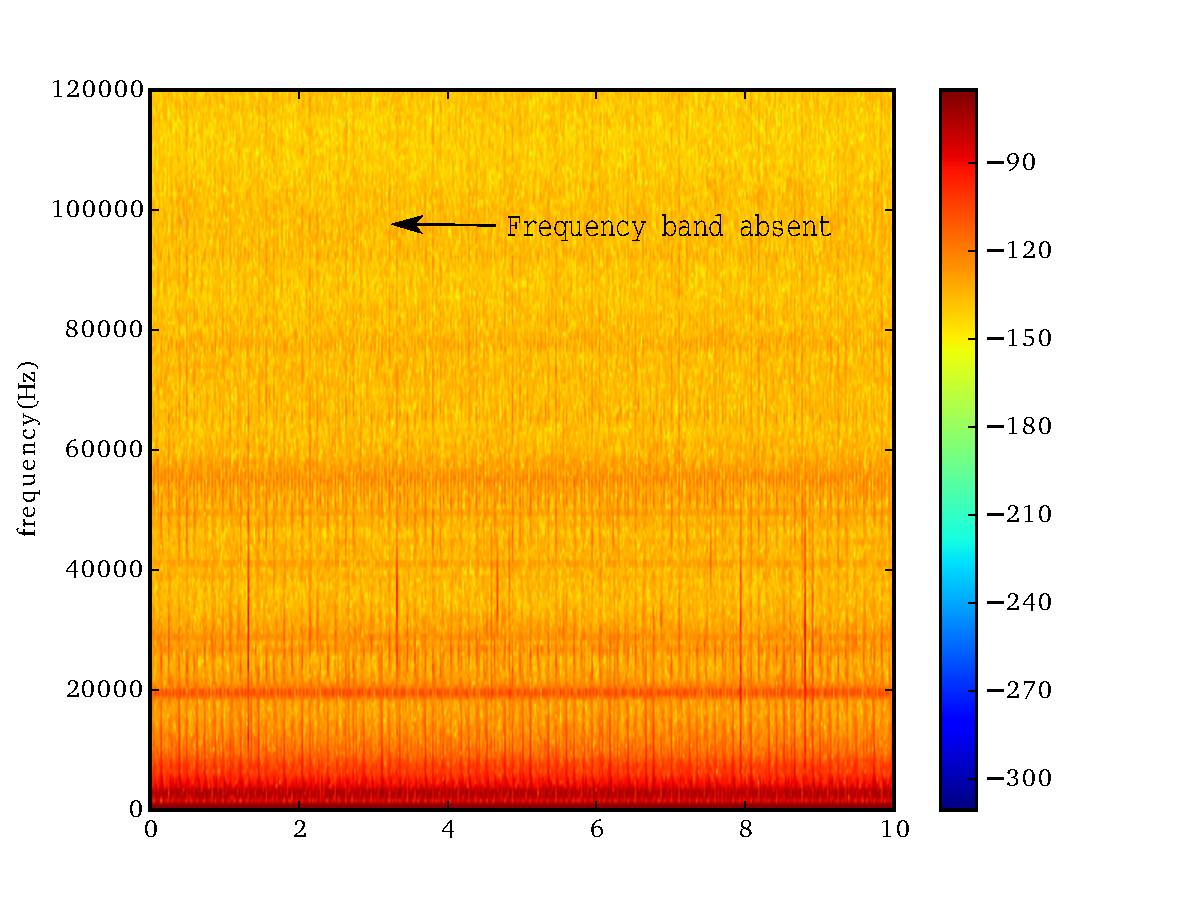
\includegraphics[width=.8\linewidth]{./figures/nest_4096/nest_standby_4096_clipped.pdf}
\caption{EMI generated by Google Nest Camera when it is playing music
  from the Internet. Fs=2.5MHz, N=4096, Fs/N=610.35}
\label{fig:nest_standby}
\end{figure}

\begin{figure}[H]
\centering
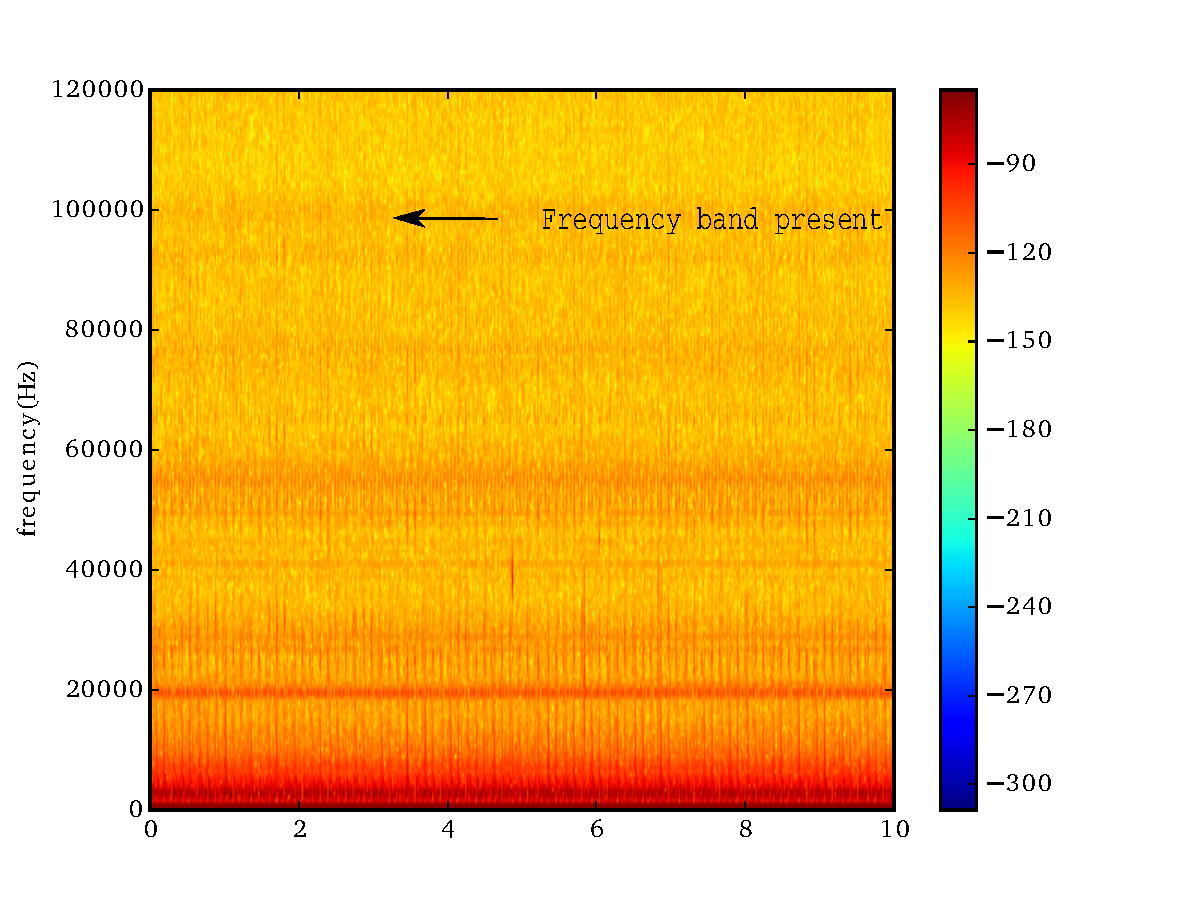
\includegraphics[width=.8\linewidth]{./figures/nest_4096/nest_stream1080_4096_clipped.pdf}
\caption{EMI generated by Google Nest Camera when it is playing music
  from the Internet. Fs=2.5MHz, N=4096, Fs/N=610.35}
\label{fig:nest_stream1080}
\end{figure}


\begin{figure}[H]
\centering
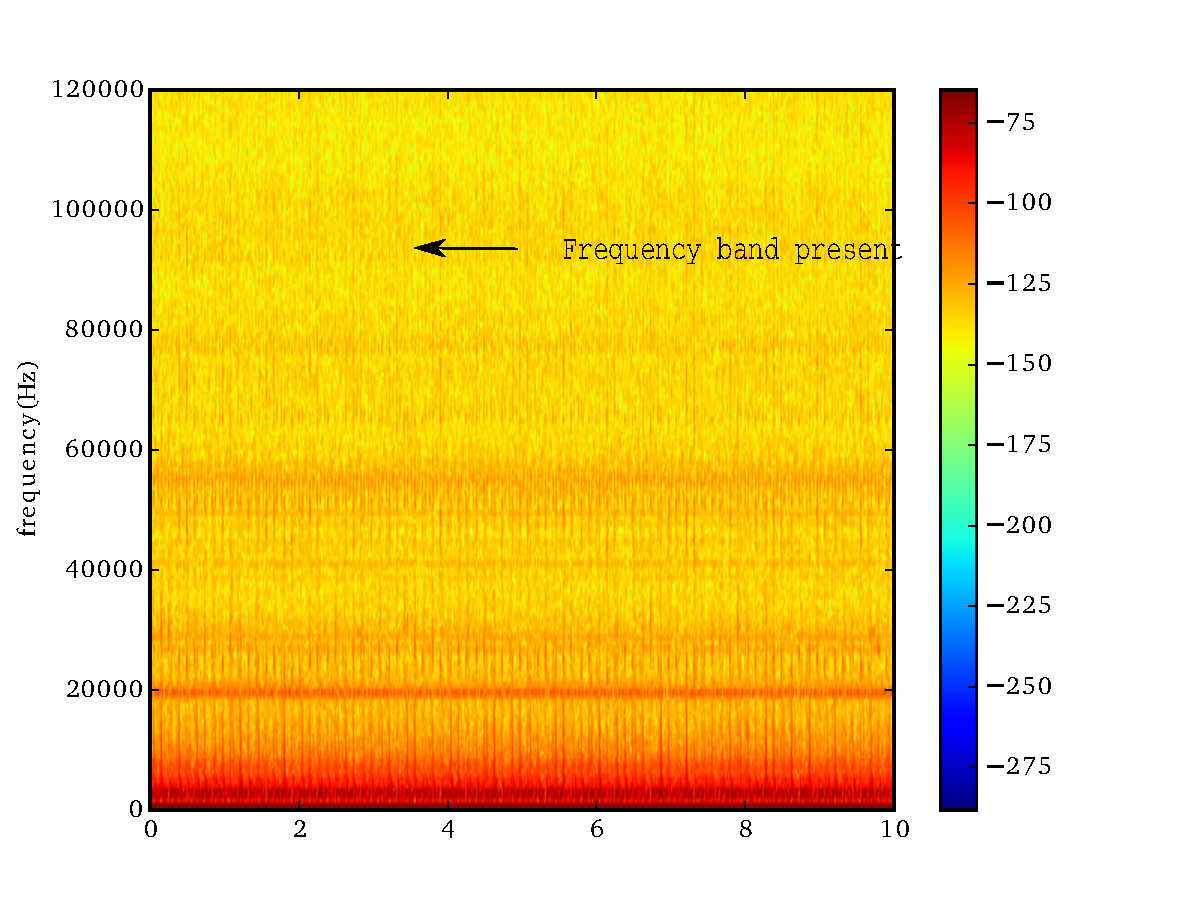
\includegraphics[width=.8\linewidth]{./figures/nest_4096/nest_stream_4096_clipped.pdf}
\caption{EMI generated by Google Nest Camera when it is playing music
  from the Internet. Fs=2.5MHz, N=4096, Fs/N=610.35}
\label{fig:nest_stream}
\end{figure}

\begin{figure}[H]
\centering
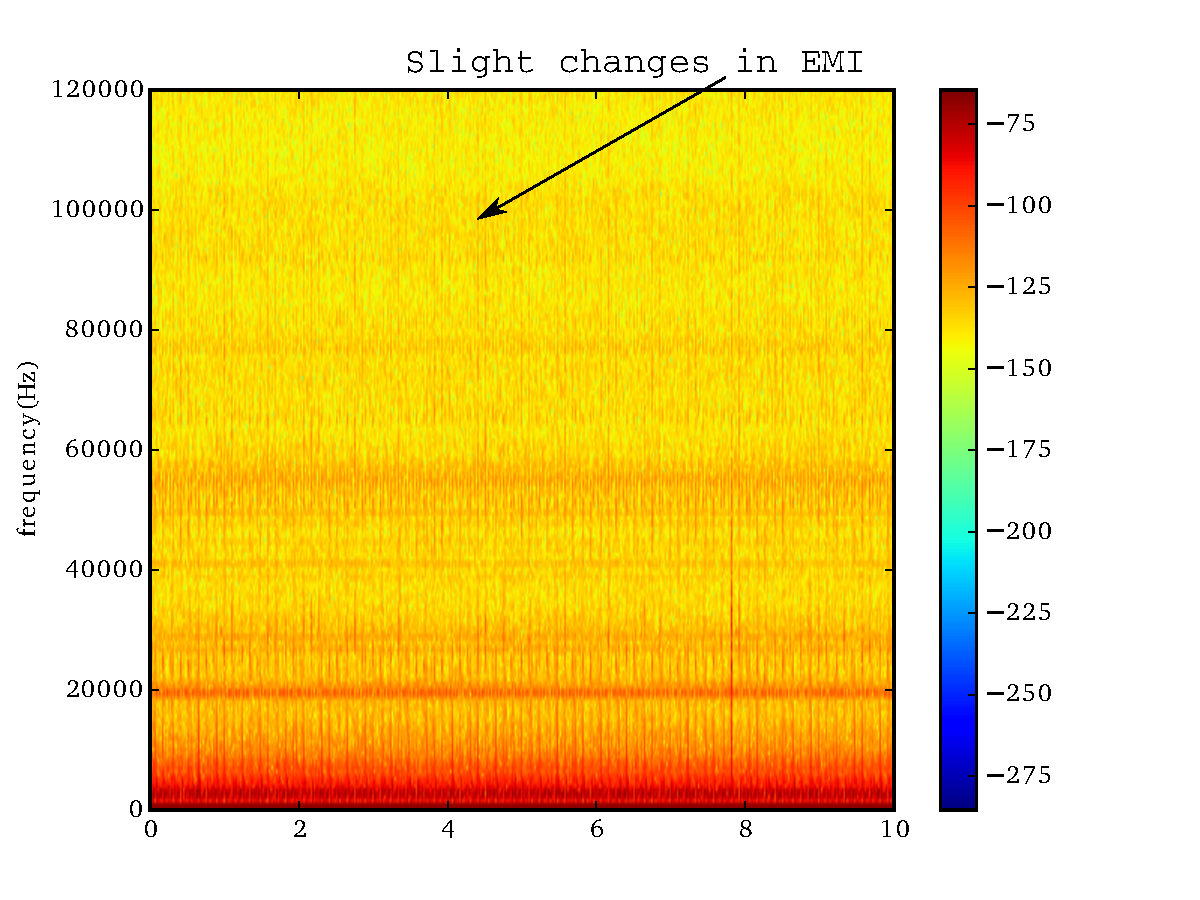
\includegraphics[width=.8\linewidth]{./figures/nest_4096/nest_stream_audio_4096_clipped.pdf}
\caption{EMI generated by Google Nest Camera when it is playing music
  from the Internet. Fs=2.5MHz, N=4096, Fs/N=610.35}
\label{fig:nest_stream_audio}
\end{figure}

\section{Alexa}
The following observations on spectrograms are worth noting:
\begin{enumerate}
\item Alexa is a fairly complex device to be modelled.
\item I think Alexa is always listening (but responds only when you
  are ask \textit{Alexa, find me XYZ}. Figure~\ref{fig:alexaMusic} and
  Figure~\ref{fig:alexaoff} suggest that due very similar EMI spectrograms.
\item There is a difference in the EMI when Alexa listens to a human
  query while possibly sending data to the Internet as in
  Figure~\ref{fig:alexaSearch}
\item I was expecting a difference when it is playing
  music (in Figure~\ref{fig:alexaMusic}) and idle (in Figure~\ref{fig:alexaoff}). I don't
  think there was a noticeable difference to the eye. First it might
  be too low energy consuming or the buffering of music content in
  buffer might have resulted in no spike. It is hard to conclude.  
\end{enumerate}

\begin{figure}[H]
\centering
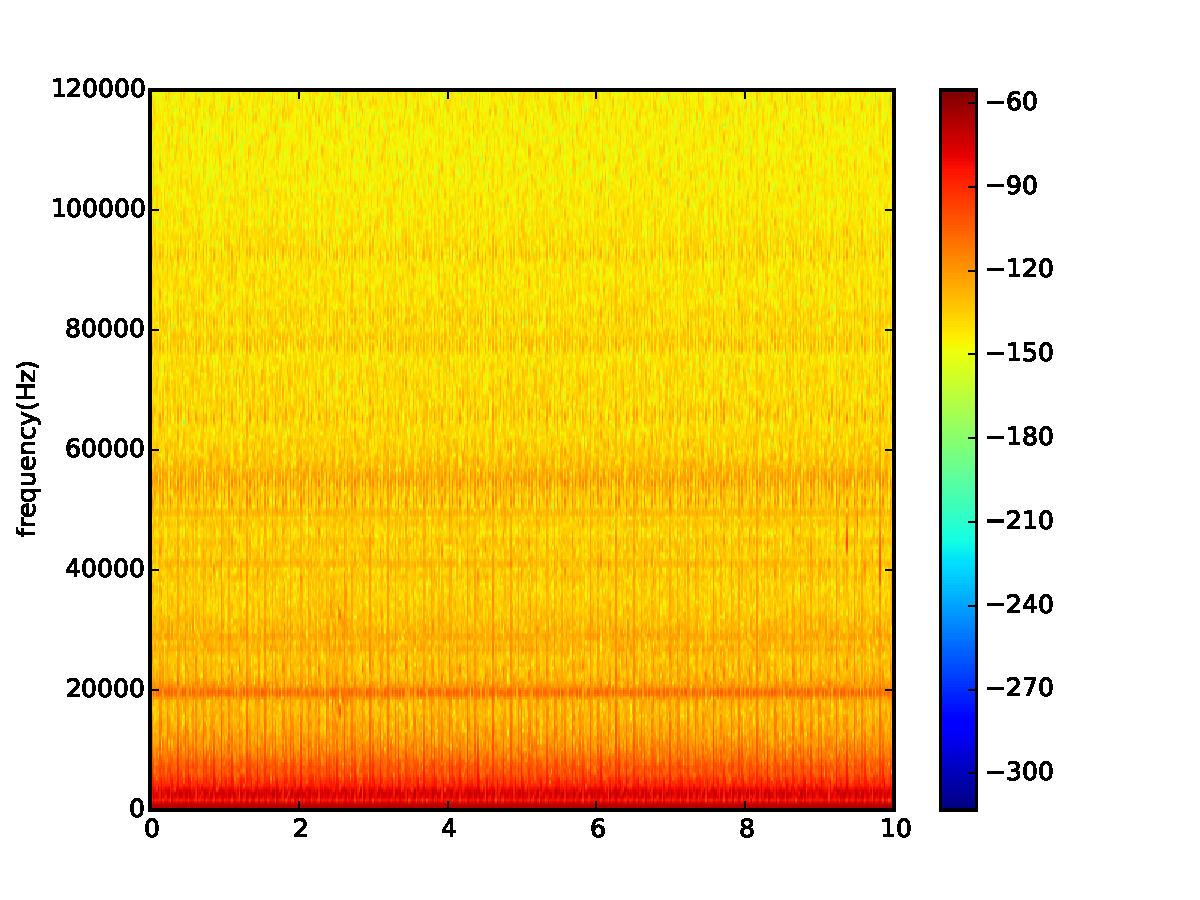
\includegraphics[width=.8\linewidth]{./figures/echo_4096/alexaMusic_4096_clipped.pdf}
\caption{EMI generated by Amazon Echo Alexa when it is playing music
  from the Internet. Fs=2.5MHz, N=4096, Fs/N=610.35}
\label{fig:alexaMusic}
\end{figure}

\begin{figure}[H]
\centering
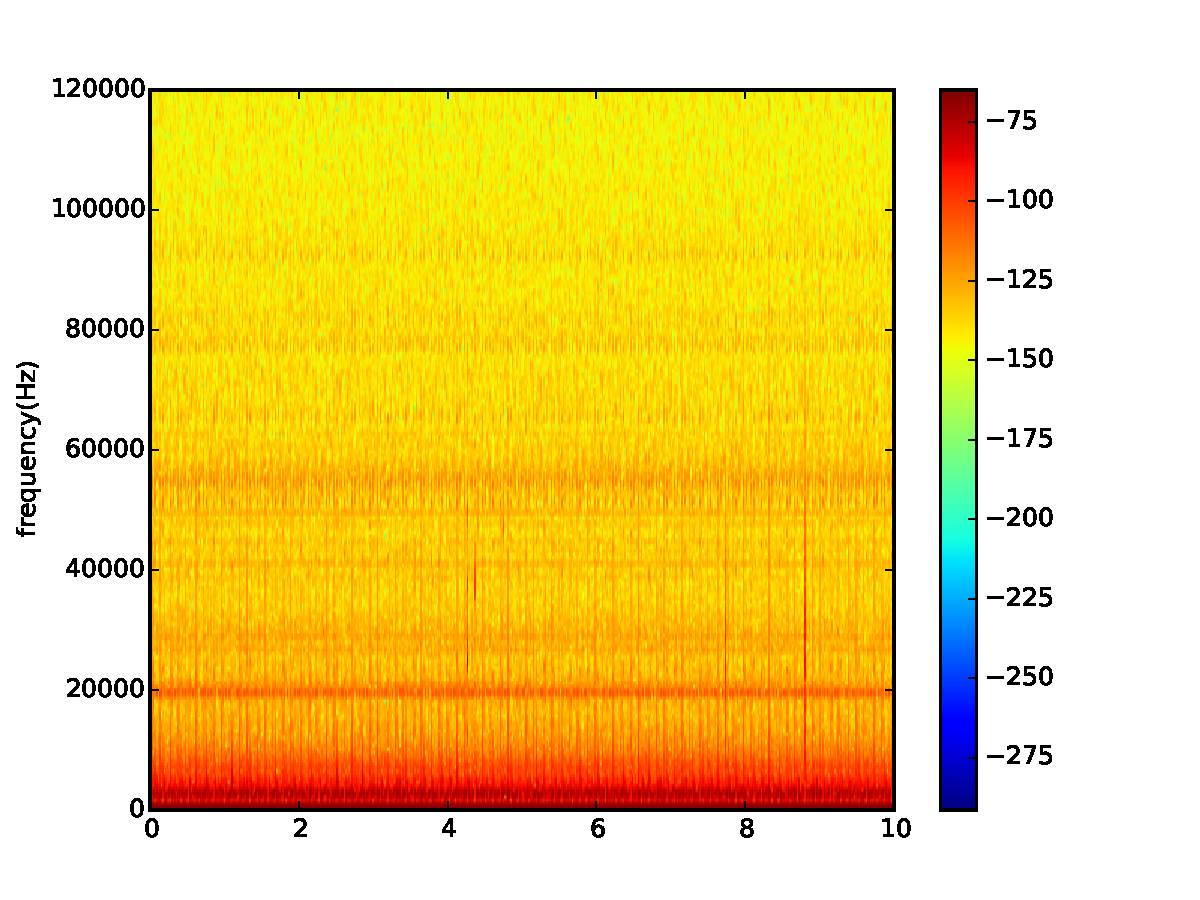
\includegraphics[width=.8\linewidth]{./figures/echo_4096/alexaOff_4096_clipped.pdf}
\caption{EMI generated by Amazon Echo Alexa when it is not asked for
  any task and is idle. Fs=2.5MHz, N=4096, Fs/N=610.35}
\label{fig:alexaoff}
\end{figure}

\begin{figure}[H]
\centering
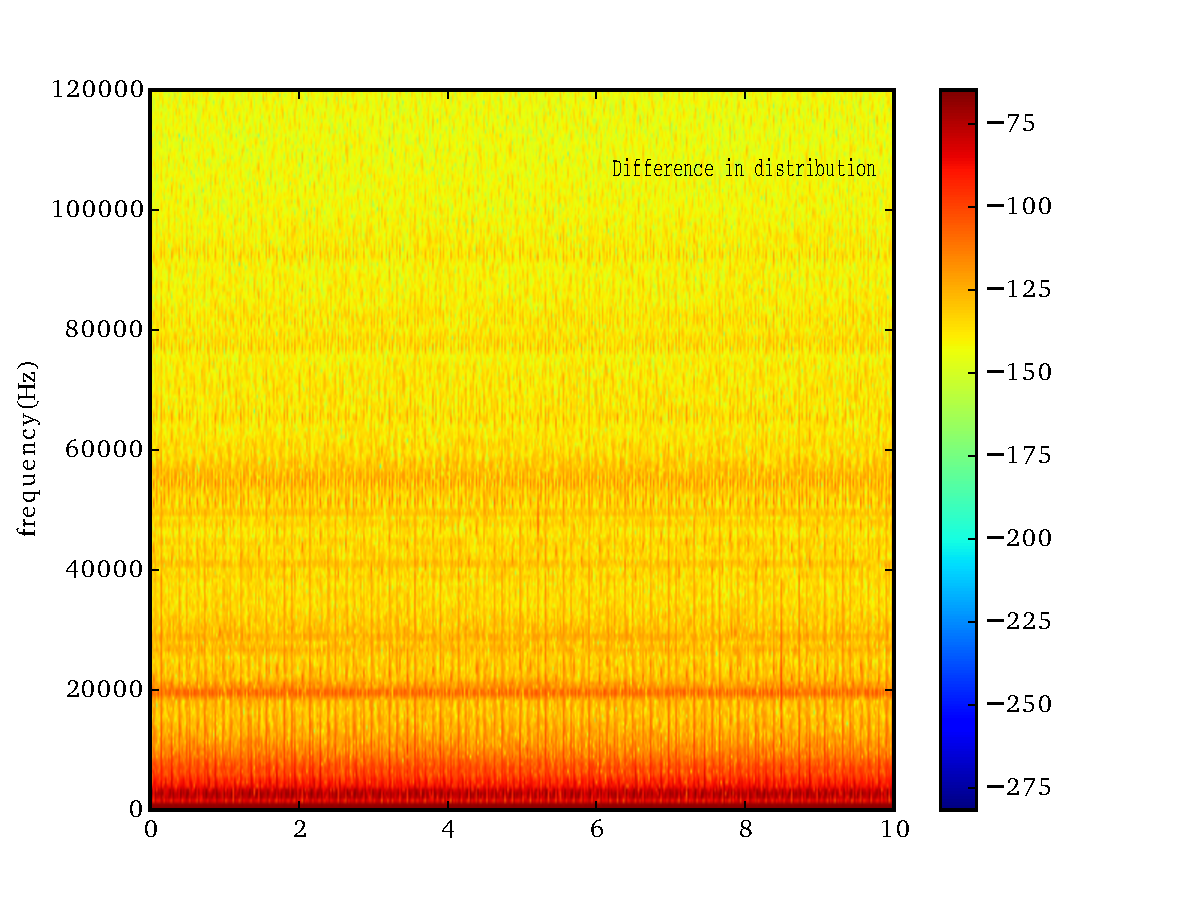
\includegraphics[width=.8\linewidth]{./figures/echo_4096/alexaSearch_4096_clipped.pdf}
\caption{EMI generated by Amazon Echo Alexa when it is listening to a
  query to search on the Internet. Fs=2.5MHz, N=4096, Fs/N=610.35}
\label{fig:alexaSearch}
\end{figure}

\section{IoT Botnet samples for Evaluation}

I have come across the following botnets infecting the IoT devices the
most.
\begin{enumerate}
\item Linux.Darlloz [4] (mines Crypto Currency such as DogeCoin, MinCoins)
\item Linux.Remaiten (CNC by actual IRC channel)
\item Linux/IRC Telnet (IRC is the CNC)
\item *Linux.Wifatch (expected to secure IoT, turned rogue)
\item Linux/Luabot (Botnet written in \textit{Lua})
\item *Linux Aidra
\end{enumerate}

I have been able to get source code for two of the starred above malwares,
They do \textbf{not} compile currently.

\begin{enumerate}
\item It has been difficult to find a working codebase like Mirai
  which can be run on OpenWrt router or Raspberry Pi for analysis
\item There are parts of the IoT malware binaries~[2,3] which are
  reversed engineered to show the exploit but are not good to run on
  raspberry or router
\item Number of malware github repositories have worms targeting
  Windows. WattsUpDoc(Kevin Fu et. al)[1] had Windows device (compounder)
  which I suppose were able to use such malwares
\item Able to run \textit{cpuminer}, a mining client for
  bitcoin/litecoin on raspberry. Unclear(shouted out
  to OpenWrt folks without response) how to port it on OpenWrt, if we
  want to run on a router
\item I contacted a reverse-engineer/hacker who pointed me to
  \textit{KernelMode.info} forum for binaries for
  \textit{Linux/LuaBot} malware. Unfortunately, I am not getting
  registered to login the forum and still waiting.
\end{enumerate}

\subsection{Mining botnets}
I have searched for different IoT botnets. There has been a specific
attack vector of mining crypto currencies on \textit{Hikvision DVR}s
in 2013-2014 while most attacks being DDoS. Currencies such as
\textit{Dogecoin, MinCoins and LiteCoin} have been mined [4] by some
bots only on x86 (not observed on ARM or MIPS architectures).

\begin{figure}[H]
\centering
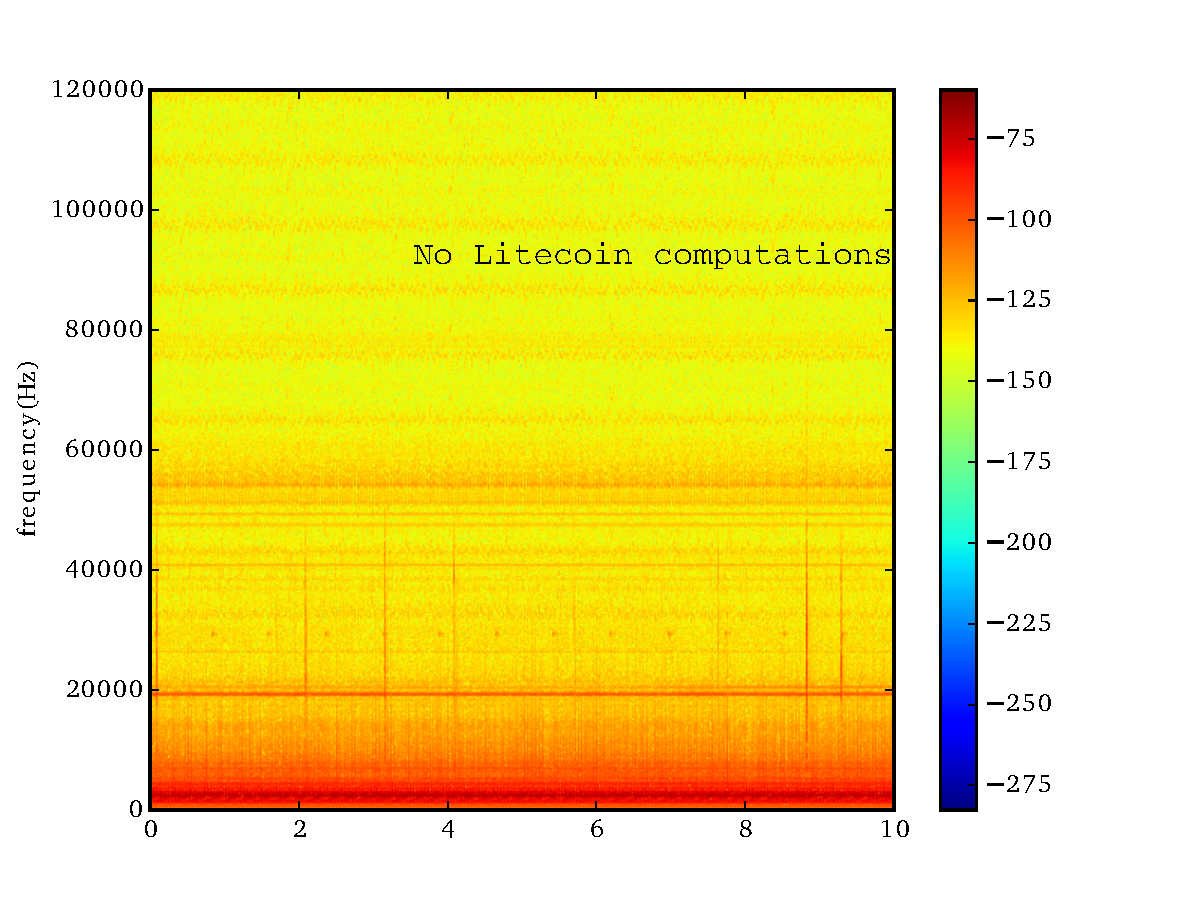
\includegraphics[width=.8\linewidth]{./figures/litecoin_stopped_4096_clipped.pdf}
\caption{Raspberry Pi Idle for baseline comparison}
\label{fig:raspi_litecoinOff}
\end{figure}

\begin{figure}[H]
\centering
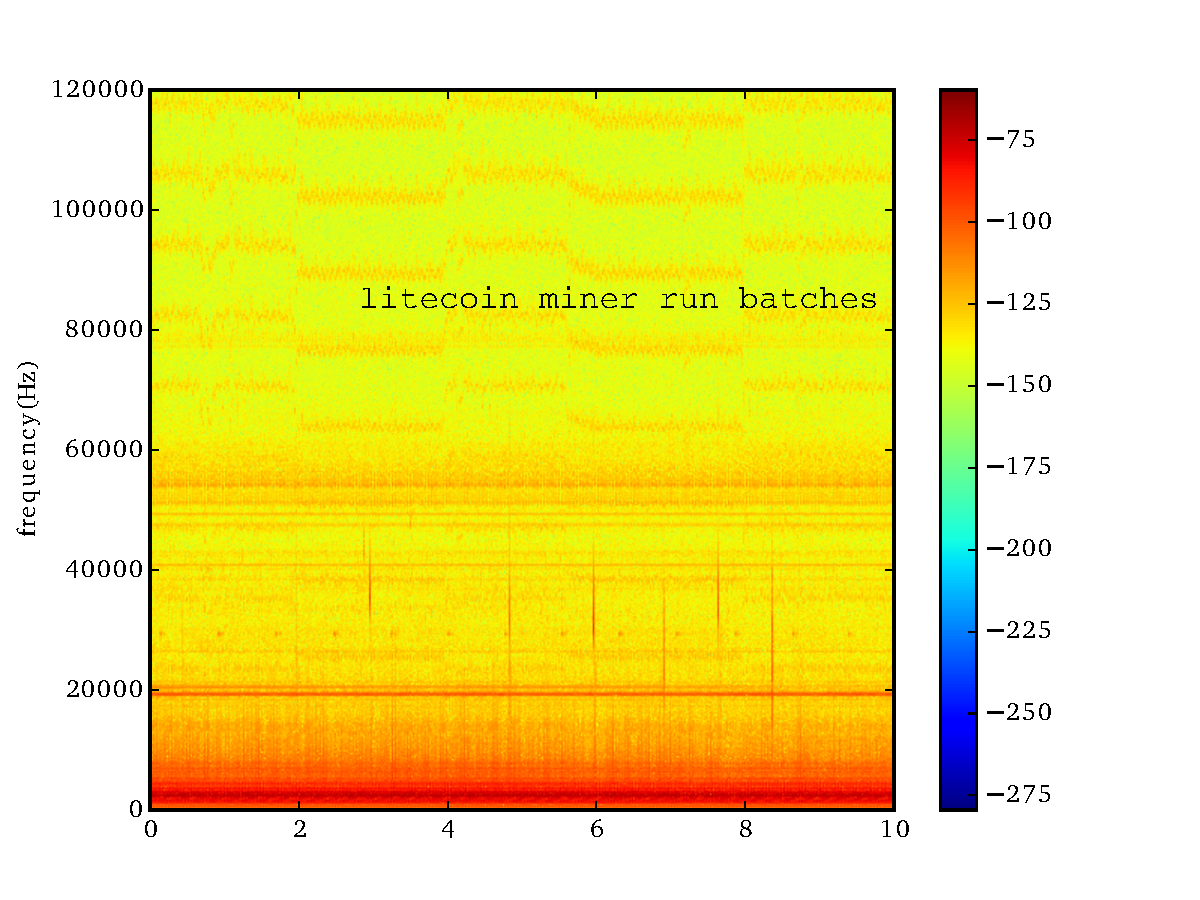
\includegraphics[width=.8\linewidth]{./figures/litecoin_working_4096_clipped.pdf}
\caption{Raspberry Pi running proof-of-work computations for
  crypto-currency using a litecoin client connected to a remote
  server}
\label{fig:raspi_litecoinOn}
\end{figure}

Figures~\ref{fig:raspi_litecoinOff},\ref{fig:raspi_litecoinOn} show the EMI
generated raspberry pi while operating cpuminer client. This is done
after waiting for a while for fetching LuaBot codebase [4].

\section{References}
\begin{enumerate}
\item https://spqr.eecs.umich.edu/papers/clark-healthtech13.pdf
\item https://w00tsec.blogspot.com/2016/09/luabot-malware-targeting-cable-modems.html
\item http://blog.malwaremustdie.org/2016/09/mmd-0057-2016-new-elf-botnet-linuxluabot.html
\item https://securityledger.com/2014/03/linux-iot-worm-still-alive-and-mining-virtual-coins/
\end{enumerate}

\section{Supplementary}
\section{Power, Current, Voltage consumed by Nest Camera}

I have borrowed this image(generated by software provided by Power
measurement equipment) from UG student working on actual
power measurements with Nest Camera. It shows good variation in Current and Energy
consumptions (voltage is not clearly indicative) when the Camera is
turned for streaming and when it is not streaming. There is clear
power draw shown in the plot but I think the Nest adapter is of good
quality to spill reasonably low EMI.
\begin{figure}[H]
\centering
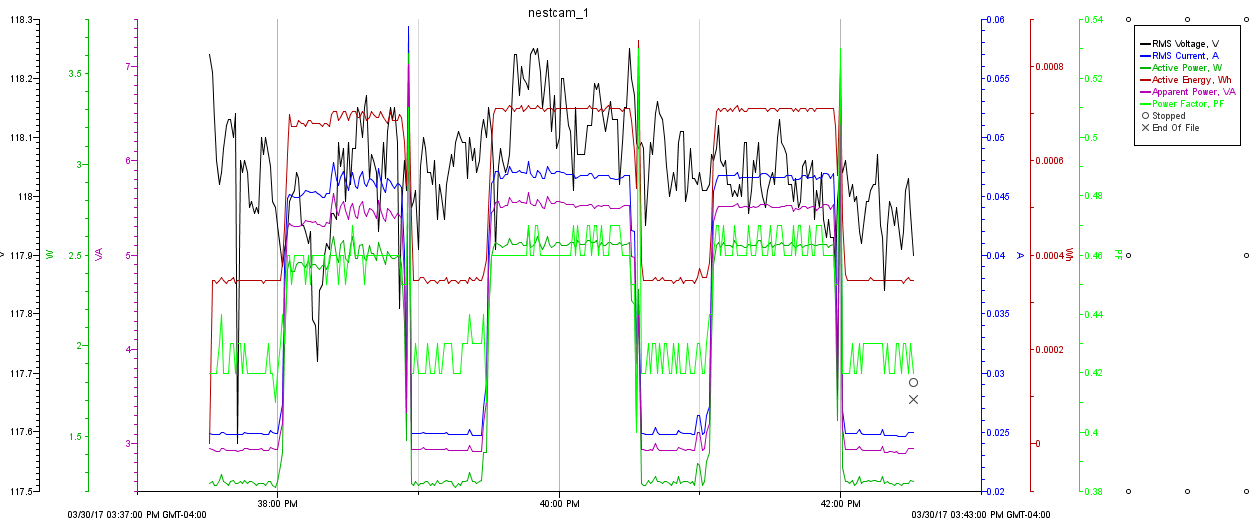
\includegraphics[width=\textwidth]{./figures/nestcam_experiment.PNG}
\caption{Actual Power consumed by Nest Camera when Turned On and
  Turned Off. Generated by experiments done by student working on
  Power Consumption project}
\label{fig:powerConNest}
\end{figure}

\subsection{Network access denied}
My wall Ethernet-port is blocked at times by Princeton Support as they
detect malware!
\begin{verbatim}
Name: pu153716
DNS Domain: student.Princeton.EDU
Entry Type: HOST
Interface[1] Type: Ethernet
Interface[1] MACaddress: e8:de:27:b7:24:4b
Interface[1] Subnet: driftnet
Interface[1] IPAddress: 172.24.63.68
System Type: OTHER
Operating System: LINUX
OIT NIS NetGroup: princetonhosts
OIT NIS NetGroup: princetonunixhosts
Technical Contact: heekang@princeton.edu
Dormnet Subscriber Netid: heekang

``Mirai is malware that turns computer systems running Linux into
remotely controlled ``bots'', that can be used as part of a botnet in
large-scale network attacks.'' en.wikipedia.org/wiki/Mirai_(malware)
\end{verbatim}

\end{document}
